\documentclass[12pt,oneside]{amsart}
\usepackage[margin=1in]{geometry} % see geometry.pdf on how to lay out the page. There's lots.
\geometry{a4paper} % or letter or a5paper or ... etc
\usepackage{graphicx}
\usepackage{listings} 
\usepackage{xcolor}
\usepackage{float}
\lstset{stepnumber=0.5, frame=single,language=c}

\title{}
\author{}

\begin{document}


\maketitle
\section{Related work}
A good example of object description using primitive shapes is \cite{pap2} however this solution is designed basing on database of CAD produced objects which is less difficult than dealing with noisy data of a point cloud. Eventhough the results obtained are relatively good, the computational time precludes using it for real time applications. In \cite{pap1} presented solution fits very well requirements of this project. The approach involves using RANSAC for primitives fitting and probabilistic graph algorithm approach for recognizing the object. Nevertheless the computational time obtained is quite high due to lack of preprocesing for the point cloud and trying to fit basic shapes on raw obtained data from kinect. Our approach is trying to decrease this time by quick preprocessing of the point cloud which allows to run RANSAC in shorter time. In addition we use a simplified graph algorithm without probabilistic approach.

\section{Object recognition module}
This section discusses algorithm used for the object recognition in \emph{lobos\_prmtv\_process} node after planes segmentation was performed. In the following subsections each step is described in details pointing out the problems and alternative approaches taken into consideration. The general pipeline followed by this module is presented on figure \ref{fig:pipeline}. However due to poor results obtained in some sections, final approach deviated slightly from the initial idea.


\begin{figure}
  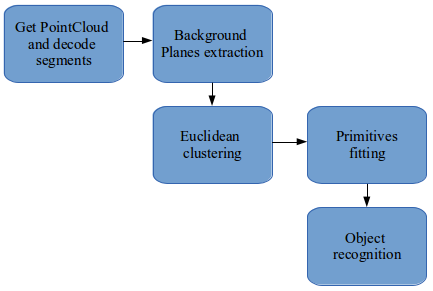
\includegraphics[scale=0.7]{images/pipeline}
  \caption{Object recognition pipeline after plane segmentation.}
  \label{fig:pipeline}
\end{figure}
\subsection{Planes decoding}
The node subscribes to topic \emph{planes\_segmented} which publishes cloud with various colors for the planes extracted. First in order to be able to work with obtained plane segments they have to be decoded. For that purpose we use a map where RGB values are considered as a key while the map value points the index of cloud in output vector. General algorithm of the function \emph{getColorSegment()} is shown on figure \ref{code:algo}.

\begin{figure}[H]
\begin{lstlisting}
for each point i in point cloud
  if in map exists key 'i.RGB'
    add i to point cloud in output vector,
    with idx == value of map for this key
  else
    create new map entry with value
    create new point cloud in output vector
    add i to created point cloud
\end{lstlisting}
\caption{Pseudo-algorithm for decoding the segments from the color cloud.}
\label{code:algo}
\end{figure}

Disadvantage of this solution is that we have to decode already segmented in other node point cloud. Modularity comes at the cost of additional computation. This simple solution was used due to the lack of appropriate message that could handle e.g. vector of point clouds. The most optimal solution would be to create ROS message able to do so. Having that, one could avoid decoding the segments, because they would be passed directly from the segmentation node.

\subsection{Plane extraction}
Objects are most commonly local areas in the point cloud scene. Therefore in order to focus just on the relevant part of the data, we extract unnecessary planes obtained in segmentation. First problem to perform this task is how to determine which planes are irrelevant for particular algorithm? It can be safely assumed that walls are least relevant segments, as well as ground floor, which however might be usefull e.g. to determine the basis of objects, calculate their height etc.
\newline
\indent Having the vector of segments we can either set a threshold for number of points in segment or remove the biggest segments assuming that floor and wall will usually cover the biggest parts of the scene. Both methods are strongly scene dependent and prone to errors in various scenes cases. We applied size threshold empirically determining the value. Using the wooden blocks, on which most of the test was performed, we applied thresholding at different levels. As a result we found that 1/10 of the total scene point cloud size is a	 threshold sufficient to maintain important parts.
\newline
\indent Obviously this is a very trivial approach tested in simple scene cases where object can be clearly distinguished. This solution would fail in case where the environment is cluttered with multiple planes or the object ocupies most of the registered cloud points. Better approach would involve determining which segment is the floor plane first and then finding planes vertical to this plane. It can be achieved using the sensor position which can be obtained in PCL. 

\subsection{Euclidean clustering}
\indent It can be observed from segmentation results that primitive parts like table legs are actually composed of few segments. Since the aim is to be able to recognize basic shapes represented by primitives these subsegments of the primitives have to be merged into one cluster. This can be achieved by euclidean clustering.
\newline
\indent In order to cluster the segments,the algorithm for given distance threshold finds the nearest neighbour for particular point and if it meets the requirements it proceeds to this point and repeats the procedure until there is no more points that can be assigned to the cluster. Since computational time is crucial, the PCL euclidean clustering uses KdTree which allows to tremendously decrease this parameter. 
\newline\newline
\indent KdTree structure + nearest neighbour search explanation if needed?
\newline\newline
Again the parameters problem arises in this case. Crucial input in case of euclidan clustering is the minimum/maximum possible size of the cluster and threshold distance between points. This will obviously vary for different input data. Size constraints for the clusters were determined again experimentally like in case of plane extraction described in previous section. Determining the distance threshold is more problematic since it will strongly depend on range at which the object was registered. Therefore the appropriate solution would be to choose this coefficient basing on the range information, however we followed less robust solution of just setting it to constant value. This significantly limits robustness of the overall algorithm because it will perform well only for object registered at certain range of distances from the sensor. 
\subsection{Primitive fitting}
Recognizing primitive shapes in the clusters gives the possibility to describe bigger(in terms of type variation) set of objects hence one is able to better process obtained data. For this purpose RANSAC algorithm was used as in \cite{pap1}. It allows to iteratively estimate a mathematical model, from a given input data. Since the considered problem requires generic detection, this solution fits perfectly. Algorithm is already provided with many basic shape models in PCL and in addition for clusters on which the tests were performed it did not influence the computational time in a significant way.
\newline
\indent The general idea of RANSAC is quite simple. Having the mathematical model it iterates through the input data and basing on predetermined threshold values it's trying to fit given point into the model thus separating inliers from outliers. The higher is the number of iterations in RANSAC that is used the better model approximation will be obtained.
\newline
\indent RANSAC however is no different than previously described parts of algorithm in terms of problems. It suffers even more from the parameters that are passed to the algorithm in order to fit the shape. The result depends on about 5 parameters(depending on the application) which are hard to determine in generic way for every scene. Problem with obtaining good results in terms of primitive shape fitting was the reason to slightly change and simplify the algorithm. Instead of using primitive shape specific descriptions, only their orientation was taken into consideration in order to divide the data into classes of of horizontal(planes) and vertical(supports) objects.  

\begin{figure}
  \begin{tabular}{|c|c|}
  \hline
  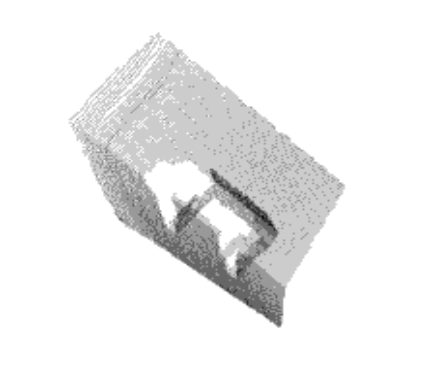
\includegraphics[scale=0.4]{images/cloud1} & 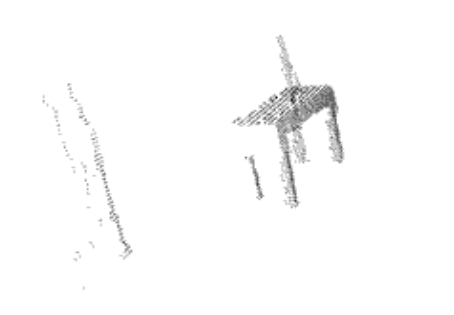
\includegraphics[scale=0.4]{images/cloud2}\\
  \hline
  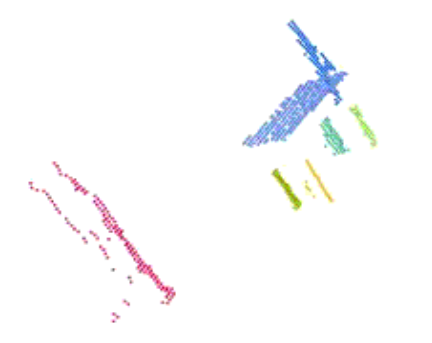
\includegraphics[scale=0.4]{images/cloud3} & 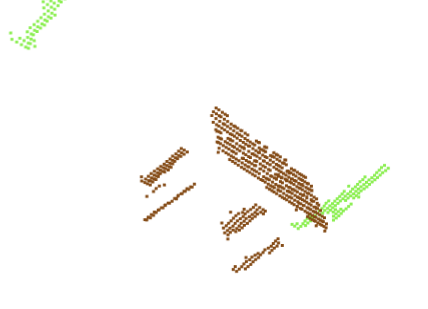
\includegraphics[scale=0.4]{images/cloud4}\\
  \hline
  \end{tabular}
  \caption{Result of the algorithm without using basic shapes fitting. Top row: original input cloud, cloud with extracted planes. Bottom row: euclidean clustering, final result with grouping}
  \label{fig:clustResult}
\end{figure}
\subsection{Primitives orientation}
Primitives orientation function \emph{getDirection()} was implemented in order to determine whether particular cluster is oriented verticaly or horizantaly. It was designed for the simplified version of object recognition due to poor results of basic shape fitting explained in previous section.\newline
\indent Function makes use of \emph{pcl::getMinMax3D()} function which for input cloud returns maximum and minimum points with respect to each axis. Taking into consideration known orientation of the sensor, one is able to determine difference between horizontal and vertical(w.r.t. sensor) max/min points of the cloud. The higher difference indicates whether cluster can be considered as vertical or horizontal. This solution is prone to errors in case where cluster has lonely point far away from the main cluster which will change the final result. However in this case this problem is neglected by applying function only after euclidean clustering which makes such a situation impossible. More generic solution for this function could be implemented by using standard deviation of the points from the main axes.

\subsection{Object recognition using graph algorithm}
Final problem of recognizing the object using obtained in the processing pipe clusters is solved with use of graph algorithm presented in \cite{graph}. The object recognition based on primitives can be simplified to finding predefined pattern in a graph where vertices are the primitives and edges are created depending on the euclidean distance between clusters. \newline
\indent The distance is calculated by function \emph{getMinDist()}. Using KdTree created for one cloud, one is able, for given input point, to quickly find the nearest point in the second cloud where the minimum distance will be the minimum distance between two clouds.\newline
\indent As mentioned previously due to poor results of basic shape recognition, the graph was implemented with use of just two types of vertices - horizontal planes and vertical supports. 'Table' object pattern is described as:
\begin{itemize}
  \item 3 vertical supports
  \item 1 horizontal plane
\end{itemize}
Search is computed with recursive algorithm. For every vertex in the graph it is recursively compared to every vertex in the object pattern graph. 
Then it compares every neighbour vertex to vertex neighbour in object pattern graph. The general representation of the graph algorithm is presented on figure \ref{graphAlg}.

\begin{figure}
  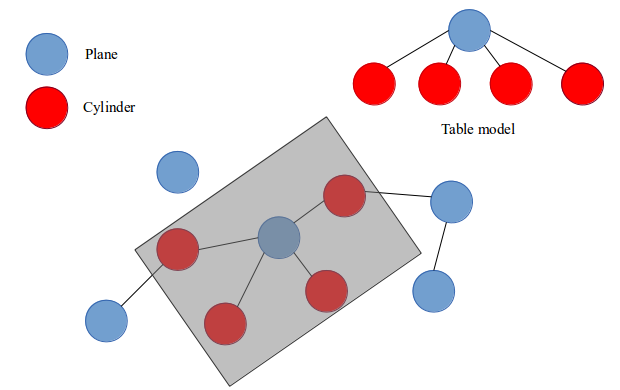
\includegraphics[scale=0.5]{images/graph}
  \caption{Simple graph algorithm visualization for table recognition problem.}
  \label{graphAlg}
\end{figure}

\section{Results}
The recognition solution was tested outside of ROS framework, on the set of 27 simple scenes(object in the middle, floor and walls) where 12 of them included table object and 15 did not. It is a small sample however taking into consideration simplicity of the scene it shows that solution does not perform really well. Results shown in figure \ref{fig:resultChart}.

\begin{figure}
  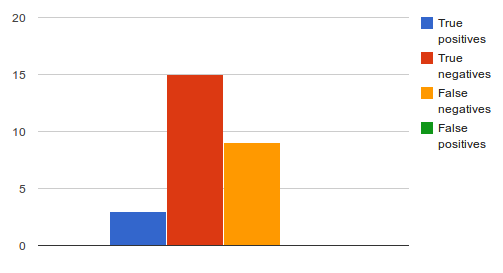
\includegraphics[scale=0.7]{images/resultChart}
  \caption{Results of applying algorithm to set of 27 simple scenes.}
  \label{fig:resultChart}
\end{figure}

Part of the false negatives results is due lack of enough vertical supports visible in the point cloud. Nevertheless taking into consideration favourable conditions of the environment one can conclude that algorithm needs to be improved. However the \textbf{average computational time} registered during this test was \textbf{1.088s} which is better than in \cite{pap1}, where on average it took 19s for object recognition.
\section{Future work \& improvements}
The final results of the implemented solution is far from being a robust one at least in the present form. It may serve as a good basis for further work. In this section main areas that should be improved are pointed out as well things that, if changed, might improve performance.
\begin{itemize}
  \item \textbf{parameters scaling} - as it was mentioned in first three sections of object recognition part, algorithms will suffer from changes in scale at which the scene is observed and this is the biggest problem of current pipeline especially when using RANSAC. It could be solved with the module which could automaticaly compute particular parameters basing on some predefined rules with respect to distance from the sensor
  \item \textbf{probabilistic graph algorithm} - once the pipeline general performance is improved so that acceptable results are obtained, probabilistic approach as in \cite{pap1} seems to be more prudent solution as long as it does not influence computational time significantly.
\end{itemize}

\section{notes}
- cloud improvement, smoothing etc, maybe reconstruction
- recognition algorithm should be improved
- problems with discarding planes 
- better primitives classification
- euclidean clustering
- KdTree
- Distance between point clouds
- clustering of spheres cylinders and planes
- ROS part, decoding the cloud
- dealing with noise
- module adjusting parameters depending on the registered cloud
- for further work in extracting planes one should think about planes that will be relevant for other applications(support in the chair for example)

\begin{thebibliography}{1}
  \bibitem{pap1} \emph{“Shape-Primitive Based Object Recognition and Grasping”} M. Nieuwenhuisen, J. Stückler, A. Berner, R. Klein, S. Behnke
  \bibitem{pap2} \emph{“Learning the Compositional Structure of Man-Made Objects for 3D Shape Retrieval”} R. Wessel and R. Klein
  \bibitem{graph} \emph{simplestcodings.blogspot.co.uk/2013/09/graphs.html}
\end{thebibliography}

\end{document}
